\section{Infrastructure}
This section will discuss the current backend and frontend services and how they are put together. Then it will propose new and better backend and frontend services that will enable the smooth operation of maintaining the website's infrastructure, development, and content. Each section will have a diagram depicting the system that creates the OMS website, comprised of the services involved and their interactions with each other. Arrows in each section depict the flow of content and information.

\subsection{Current Infrastructure Plan}
Our current infrastructure uses GoDaddy as an End-To-End (E2E) solution. An E2E system accommodates for both ends of the website spectrum, from the people writing the content, to the people publishing the content, to the people running the website, and finally to the people reading the content.

\begin{figure}[h]
    \centering
    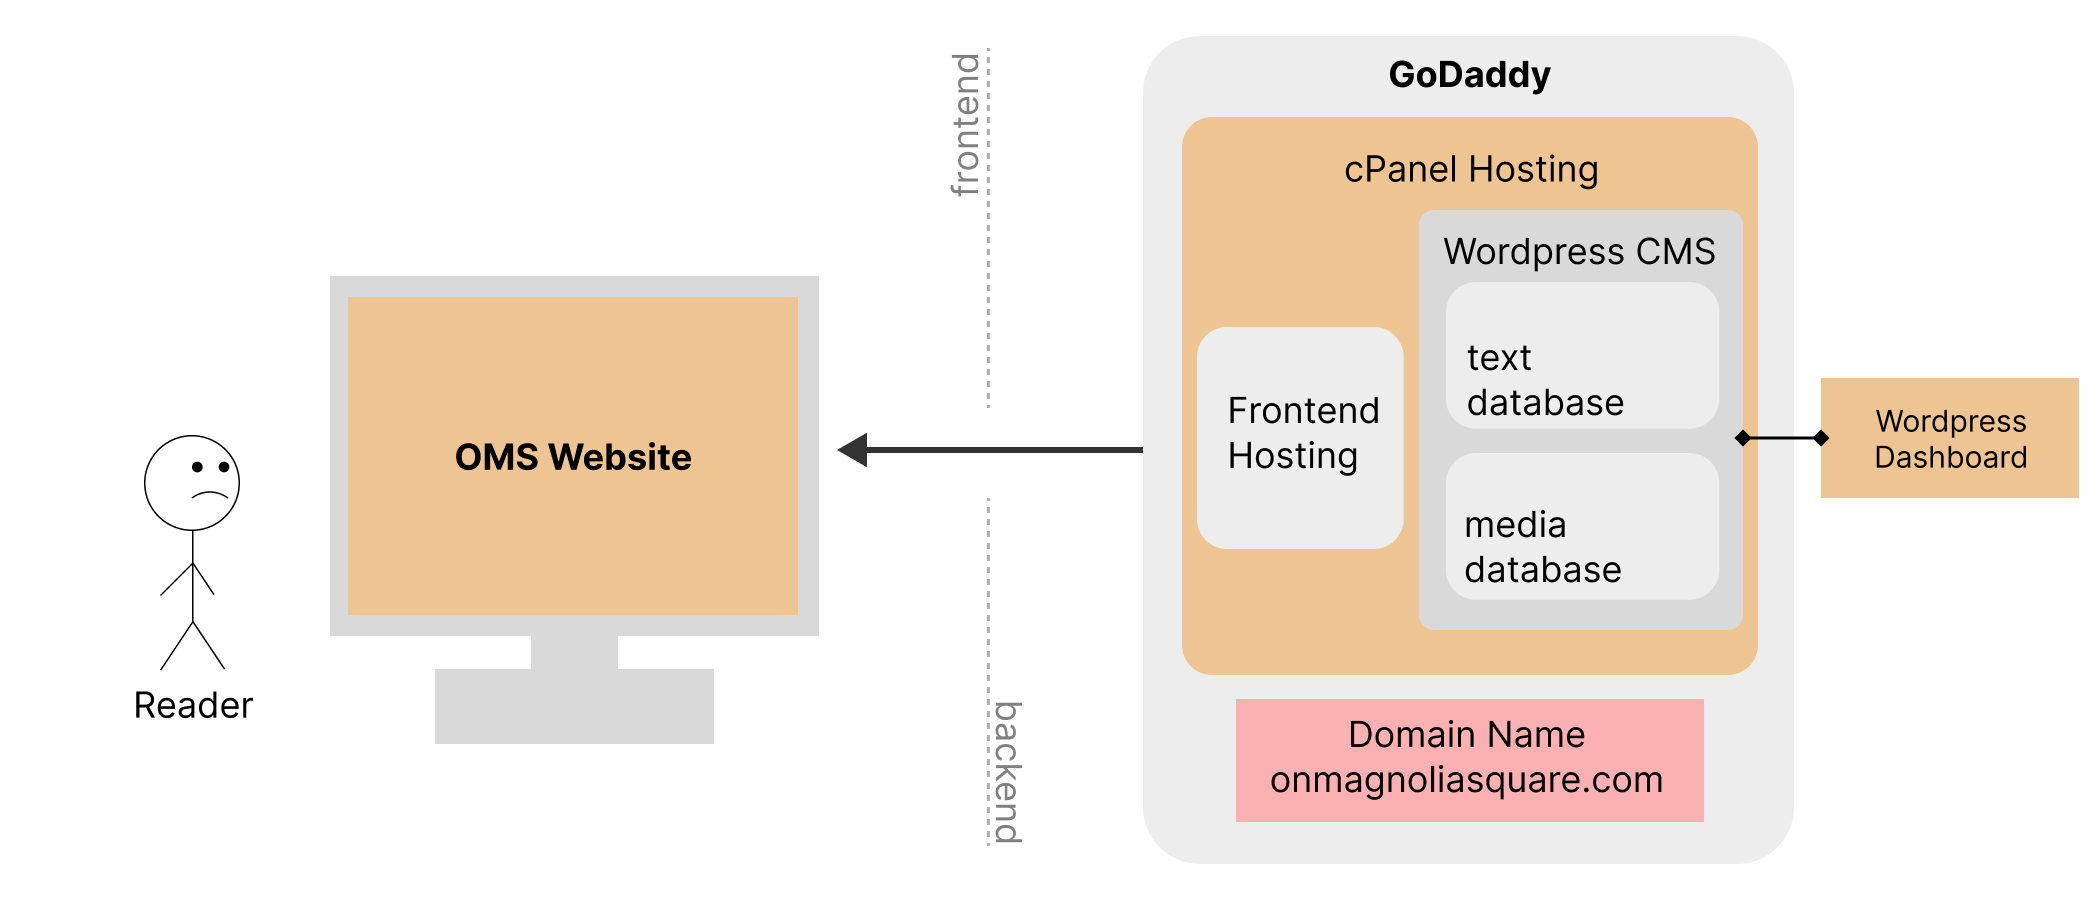
\includegraphics[scale=0.4]{diagrams/Frame 1.png}
    \caption{An End-To-End (E2E) infrastructure plan.}
    \label{fig:frame1}
\end{figure}

I suppose E2E infrastructure was implemented because every service is consolidated under one provider, in this case GoDaddy, and that makes it a one-stop-shop for everything, begetting convenience for simple content management, but it is prone to vendor lock-in and rigidity. Both vendor lock-in and rigidity violate the accessibility, robustness, and future-proofing qualities covered in §2.2.

bloated wordpress cms.

\subsection{Proposed Infrastructure Plan}

\begin{figure}[h]
    \centering
    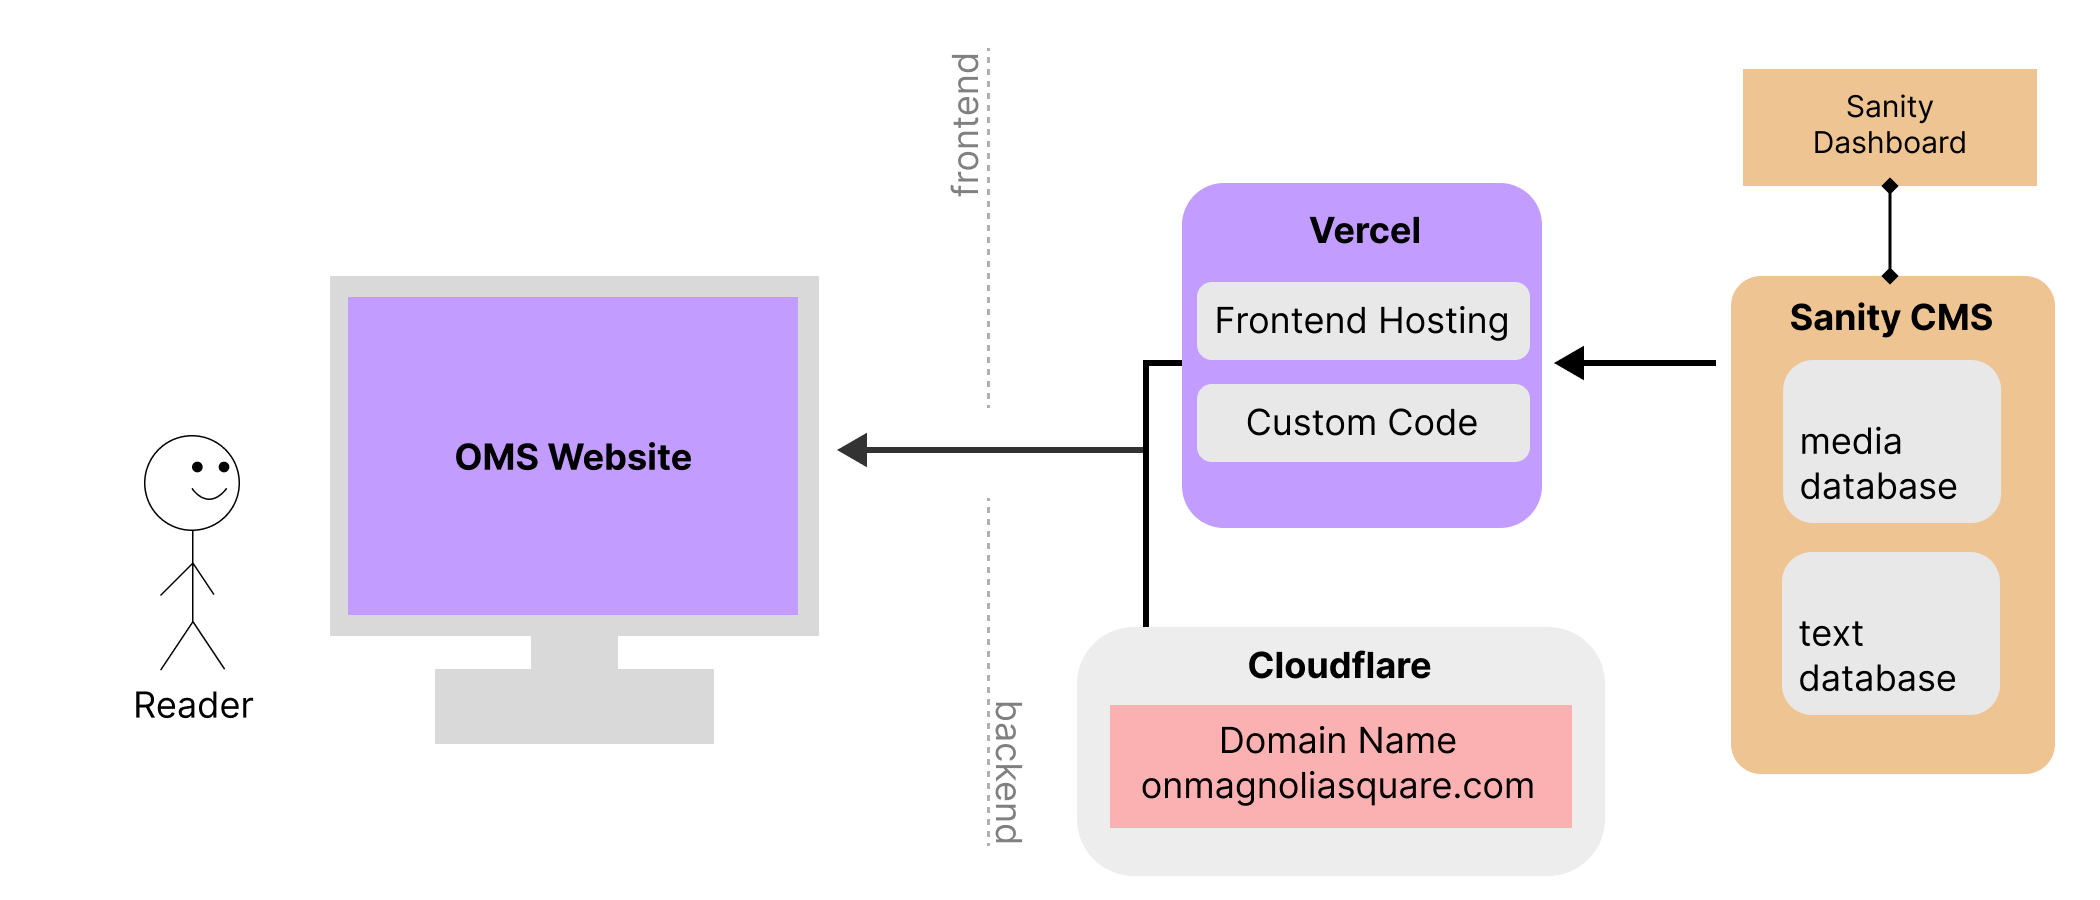
\includegraphics[scale=0.4]{diagrams/Frame 2.png}
    \caption{A best-of-breed infrastructure.}
    \label{fig:frame2}
\end{figure}

My proposed infrastructure uses a Best-Of-Breed (BOB) solution. A BOB system is like composing a three-piece suit from materials sourced from the best silk and cotton mills; every component that constitutes the website is the crème de la crème, or for our purposes, the ones that suit our requirements the best. Figure~\ref{fig:frame2} diagrams the three main services I propose to use: Cloudflare, Vercel, and Sanity.

\subsection{Proposed Services and Tools}

\subsection{Cloudflare}
Cloudflare is a company that services and maintains digital cloud infrastructure across the globe. Cloudflare has good qualities in the three trait categories. Cloudflare is accessible: the UI/UX is simple and clear. Access to different settings and functions is clearly labeled. In the event that something may be unclear, their \href{https://developers.cloudflare.com}{online documentation}\footnote{https://developers.cloudflare.com} and \href{https://blog.cloudflare.com/}{blog}\footnote{https://blog.cloudflare.com} is accessible and digestible. The services they provide are robust, dependable, and future-proof because a sizable majority of the internet flows through their worldwide data centers. Simply put, cloud security and internet infrastructure is their domain.

Because of this, they provide backend service products we're particularly interested in, such as their registrar and photo storage.


\subsubsection*{Domain Registrar}
Compared to our current registrar GoDaddy, Cloudflare's product named `Registrar' is superior in many ways.

Please note that readers who view the website will be unaware of this registrar switch – visiting the OMS URL will still display the same website content before the switch. It does not affect the frontend.

\subsubsection*{Image Storage and Hosting}

\subsubsection*{Price Breakdown}

\subsection{Sanity.io}

\subsection{Vercel}
